\chapter{Vision for Aircraft Manufacturing Automation}
\label{sec:VisionForAircraftManufacturingAutomation}

%%% Citation
\begin{flushright}
{
%\textit{"The problems of the world cannot possibly be solved by skeptics or cynics \\ whose horizons are limited by the obvious realities. We need men who can  \\ dream of things that never were and ask why not?"}
\textit{"We need men who can dream of things that never were and ask why not?"}\\
  -- \emph{John F. Kennedy}
%
%\emph{John F. Kennedy}
}
\end{flushright}
\vspace{+10pt}
%%%%

This chapter illustrates robotic concepts to automate the manufacturing of large assemblies, such as airplanes, ships, buildings, etc. For those types of manufacturing tasks robots must be able to go inside the large manufactured object, unlike car production for instance where the part can be on an assembly line and surrounded by robots.%Additionally, with typically slower rates of production and larger numbers of distinct required operations, 


\section{Current situation}
\label{sec:CurrentSituation}

%Here, the current manufacturing approach and the challenge for automating the manufacturing and assembly of aircraft is briefly explored.

In the aerospace industry, one technical challenge for the automation of aircraft manufacturing is bringing robots inside the fuselage. Currently aircraft manufacturing is dependent on highly qualified manual labor because of the complexity of tasks involved and the difficulty for accessing manufacturing sites. Currently, many temporary assemblies such as scaffolds are used to assist human workers accessing the manufacturing sites. Hence, traditional robotics systems hardly fit this type of environment; industrial robot arms are to heavy and bulky to be used effectively inside the fuselage \cite{parietti_supernumerary_2014} \cite{menon_design_2011}. 

\section{Solution Concepts}

Fig. \ref{fig:spyder} illustrate two possible solutions: one is a long, snake-like articulated arm \cite{buckingham_r._chitrakaran_v._conkie_r._ferguson_g._et_al._snake-arm_2007} and the other is a mobile robotic platform. In both cases the robot must bear the weight of its own actuation system, which increases exponentially along the serial linkage as the number of DoF increases. The use of variable gear-ratio actuator systems would solve or alleviate the actuator problem. Cu


\subsection{Light-weight long manipulator arms}
\label{sec:LightWeightLongManipulatorArm}

Alternatively, robotic arm that would be very long and articulated could be able to reach manufacturing sites from the outside of the fuselage. 

\begin{figure}[H]
	\centering
		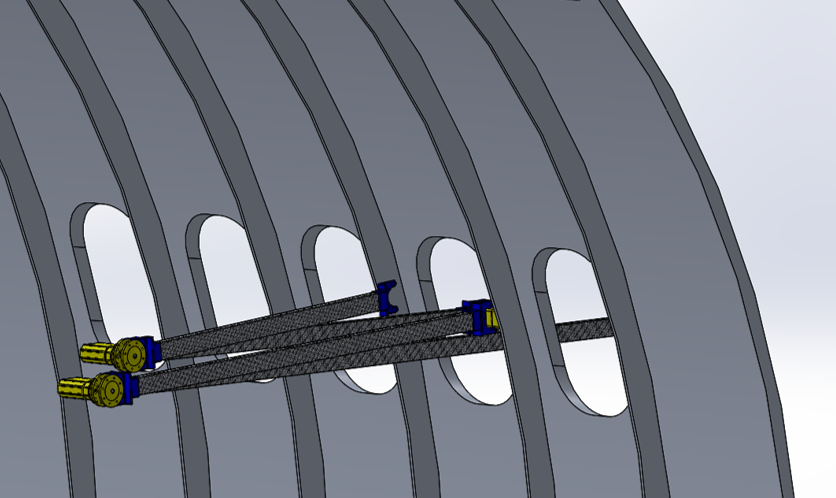
\includegraphics[width=1.00\textwidth]{arm_concept.png}
		\caption{Long light-weight arm concept for interior access}
	\label{fig:arm_concept}
\end{figure}


\subsection{Wearable robots}
\label{sec:WearableRobots}

One possible solution, to solve bring robot on site easily is to use the help of humans, which unlike robot would have no problems navigating and moving inside a manufacturing site.

\begin{figure}[H]
	\centering
		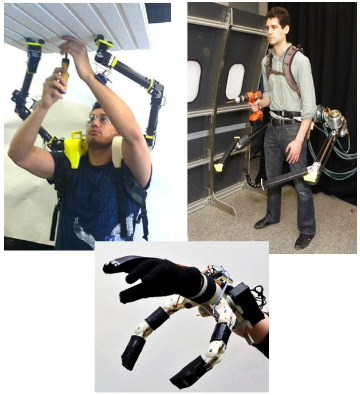
\includegraphics[width=0.6\textwidth]{wearables_robots.png}
		\caption{Wearable robot concepts and prototypes}
	\label{fig:wearable_concept}
\end{figure}



\subsection{Mobile climbing robots}
\label{sec:MobileClimbingRobots}

Another approach, aiming at a higher level of automation, is to have mobile robots walking or climbing inside the aircraft fuselage to reach manufacturing sites automatically. 


\begin{figure}[H]
	\centering
		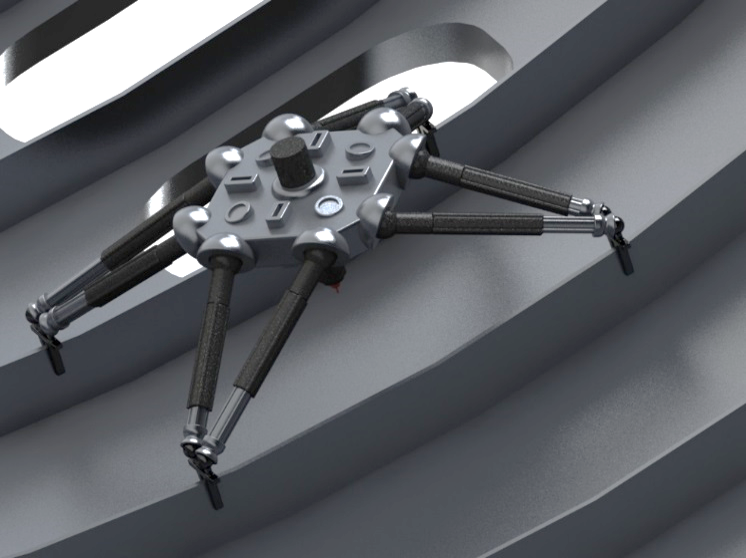
\includegraphics[width=0.9\textwidth]{spyder_concept.png}
		\caption{Mobile climbing manufacturing robot concept}
	\label{fig:arm_concept}
\end{figure}


\section{Technical challenges}